\chapter{Crear modelo relacionado}

Siguiendo con nuestro blog, donde ya tenemos una aplicación donde crear posts sólo si estamos logueado, es buen momento de añadir nuevas características. Vamos a incluir la opción de tener comentarios, al menos a nivel relacional.

Sin entrar en los atributos que tiene cada entidad/modelo, la relación que tienen los comentarios respecto a un \textit{post} sería la siguiente:

\begin{center}
    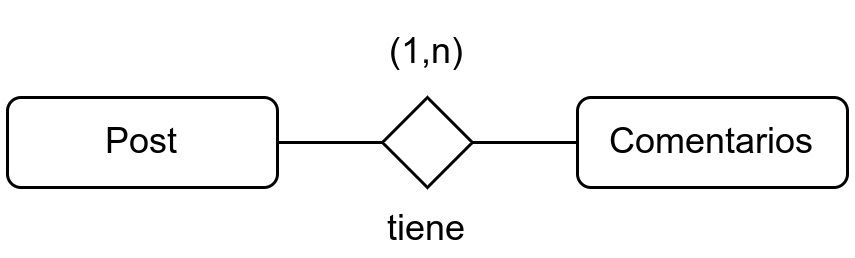
\includegraphics[width=0.5\linewidth]{e-r.png}
\end{center}

Es decir, un \textit{post} puede tener muchos comentarios. Un comentario sólo puede pertenecer a un \textit{post}. En principio el único atributo que vamos a permitir es el propio comentario, aparte de la fecha de creación. Para crear el modelo haríamos:

\begin{mycode}{Crear Modelo}{console}{{\small }}
root@1b29e46c10ae:/var/www/html# php artisan make:model Comentario -crms
\end{mycode}


\chapter{Crear migración}
Al igual que vimos al inicio, este comando nos ha creado el modelo, el controlador de \textit{resource}, el sistema de migración y el fichero para añadir la semilla a la base de datos. A la hora de generar la tabla, tenemos que hacer referencia a qué \textit{post} pertenece el comentario, por lo tanto el \textit{migration} queda:

\begin{mycode}{Crear migration}{php}{}
<?php
//...
public function up(): void{
    Schema::create('comentarios', function (Blueprint $table) {
        $table->id();
        $table->string('texto');
        $table->unsignedBigInteger('post_id');
        $table->foreign('post_id')->references('id')->on('posts');
        $table->timestamps();
    });
}
\end{mycode}

Tal como se puede ver, a la hora de crear la tabla en el \textit{migration} se ha creado un campo llamado “\textbf{post\_id}” que después se le ha indicado que es de tipo “clave foránea”. En la \href{https://laravel.com/docs/10.x/migrations#foreign-key-constraints}{documentación} se explican distintas opciones para este tipo de casos.

\exercisebox{\textbf{Crea un “seed” para añadir un comentario al primer \textit{post}}}

\chapter{Crear relación de modelos}

Hasta ahora la relación se ha creado a nivel de base de datos, pero es necesario que Laravel a nivel de \textit{framework}, mientras programamos, sea consciente de que los modelos están relacionados entre sí. Para ello, una vez más en la \href{https://laravel.com/docs/10.x/eloquent-relationships#one-to-many}{documentación} se puede ver cómo Eloquent hace uso de los distintos tipos de relaciones.

Para ello, deberemos modificar ambos ficheros de los modelos que entran en juego en esta relación:
\begin{itemize}
    \item Relación “\textbf{uno a muchos}”, donde un \textit{post} puede tener muchos comentarios. Modificaremos el modelo \configfile{App/Models/Post.php} para que contenga:
\begin{mycode}{Añadir relación “uno a muchos” en Post}{php}{}
<?php
//...
use Illuminate\Database\Eloquent\Relations\HasMany;
class Post extends Model{
    use HasFactory;
    public function comentarios(): HasMany {
        return $this->hasMany(Comentario::class);
    }
}
\end{mycode}

    \item Relación inversa “\textit{\textbf{BelongsTo}}”, donde un comentario pertenece a un \textit{post}. En este caso, modificaremos el modelo \configfile{App/Models/Comentario.php}.

\begin{mycode}{Añadir relación inversa en Comentario}{php}{}
<?php
//...
use Illuminate\Database\Eloquent\Relations\BelongsTo;

class Comentario extends Model{
    use HasFactory;
    public function post(): BelongsTo{
        return $this->belongsTo(Post::class);
    }
}
\end{mycode}
\end{itemize}

Tras esto, ya sea a través de una acción o desde Tinker, podremos obtener los comentarios de un \textit{post} específico, perfecto para dibujarlos en la vista donde se visualiza el \textit{post}. Y al revés, dado un comentario, obtener a qué \textit{post} pertenece.